\documentclass[twoside]{book}

% Packages required by doxygen
\usepackage{calc}
\usepackage{doxygen}
\usepackage{graphicx}
\usepackage[utf8]{inputenc}
\usepackage{makeidx}
\usepackage{multicol}
\usepackage{multirow}
\usepackage{textcomp}
\usepackage[table]{xcolor}

% Font selection
\usepackage[T1]{fontenc}
\usepackage{mathptmx}
\usepackage[scaled=.90]{helvet}
\usepackage{courier}
\usepackage{amssymb}
\usepackage{sectsty}
\renewcommand{\familydefault}{\sfdefault}
\allsectionsfont{%
  \fontseries{bc}\selectfont%
  \color{darkgray}%
}
\renewcommand{\DoxyLabelFont}{%
  \fontseries{bc}\selectfont%
  \color{darkgray}%
}

% Page & text layout
\usepackage{geometry}
\geometry{%
  a4paper,%
  top=2.5cm,%
  bottom=2.5cm,%
  left=2.5cm,%
  right=2.5cm%
}
\tolerance=750
\hfuzz=15pt
\hbadness=750
\setlength{\emergencystretch}{15pt}
\setlength{\parindent}{0cm}
\setlength{\parskip}{0.2cm}
\makeatletter
\renewcommand{\paragraph}{%
  \@startsection{paragraph}{4}{0ex}{-1.0ex}{1.0ex}{%
    \normalfont\normalsize\bfseries\SS@parafont%
  }%
}
\renewcommand{\subparagraph}{%
  \@startsection{subparagraph}{5}{0ex}{-1.0ex}{1.0ex}{%
    \normalfont\normalsize\bfseries\SS@subparafont%
  }%
}
\makeatother

% Headers & footers
\usepackage{fancyhdr}
\pagestyle{fancyplain}
\fancyhead[LE]{\fancyplain{}{\bfseries\thepage}}
\fancyhead[CE]{\fancyplain{}{}}
\fancyhead[RE]{\fancyplain{}{\bfseries\leftmark}}
\fancyhead[LO]{\fancyplain{}{\bfseries\rightmark}}
\fancyhead[CO]{\fancyplain{}{}}
\fancyhead[RO]{\fancyplain{}{\bfseries\thepage}}
\fancyfoot[LE]{\fancyplain{}{}}
\fancyfoot[CE]{\fancyplain{}{}}
\fancyfoot[RE]{\fancyplain{}{\bfseries\scriptsize Generated on Thu Nov 5 2020 16\-:39\-:18 for Project3 by Doxygen }}
\fancyfoot[LO]{\fancyplain{}{\bfseries\scriptsize Generated on Thu Nov 5 2020 16\-:39\-:18 for Project3 by Doxygen }}
\fancyfoot[CO]{\fancyplain{}{}}
\fancyfoot[RO]{\fancyplain{}{}}
\renewcommand{\footrulewidth}{0.4pt}
\renewcommand{\chaptermark}[1]{%
  \markboth{#1}{}%
}
\renewcommand{\sectionmark}[1]{%
  \markright{\thesection\ #1}%
}

% Indices & bibliography
\usepackage{natbib}
\usepackage[titles]{tocloft}
\setcounter{tocdepth}{3}
\setcounter{secnumdepth}{5}
\makeindex

% Hyperlinks (required, but should be loaded last)
\usepackage{ifpdf}
\ifpdf
  \usepackage[pdftex,pagebackref=true]{hyperref}
\else
  \usepackage[ps2pdf,pagebackref=true]{hyperref}
\fi
\hypersetup{%
  colorlinks=true,%
  linkcolor=blue,%
  citecolor=blue,%
  unicode%
}

% Custom commands
\newcommand{\clearemptydoublepage}{%
  \newpage{\pagestyle{empty}\cleardoublepage}%
}


%===== C O N T E N T S =====

\begin{document}

% Titlepage & ToC
\hypersetup{pageanchor=false}
\pagenumbering{roman}
\begin{titlepage}
\vspace*{7cm}
\begin{center}%
{\Large Project3 }\\
\vspace*{1cm}
{\large Generated by Doxygen 1.8.5}\\
\vspace*{0.5cm}
{\small Thu Nov 5 2020 16:39:18}\\
\end{center}
\end{titlepage}
\clearemptydoublepage
\tableofcontents
\clearemptydoublepage
\pagenumbering{arabic}
\hypersetup{pageanchor=true}

%--- Begin generated contents ---
\chapter{Hierarchical Index}
\section{Class Hierarchy}
This inheritance list is sorted roughly, but not completely, alphabetically\-:\begin{DoxyCompactList}
\item \contentsline{section}{C\-Linked\-List$<$ elt\-Type $>$}{\pageref{classCLinkedList}}{}
\item \contentsline{section}{C\-Linked\-List$<$ Word\-Data $>$}{\pageref{classCLinkedList}}{}
\item \contentsline{section}{C\-List\-Itr$<$ elt\-Type $>$}{\pageref{classCListItr}}{}
\item \contentsline{section}{node$<$ elt\-Type $>$}{\pageref{classnode}}{}
\item \contentsline{section}{node$<$ Word\-Data $>$}{\pageref{classnode}}{}
\item \contentsline{section}{Word\-Data}{\pageref{classWordData}}{}
\item \contentsline{section}{Word\-List}{\pageref{classWordList}}{}
\begin{DoxyCompactList}
\item \contentsline{section}{Word\-C\-List}{\pageref{classWordCList}}{}
\item \contentsline{section}{Word\-Data\-List}{\pageref{classWordDataList}}{}
\item \contentsline{section}{Word\-Vector\-List}{\pageref{classWordVectorList}}{}
\end{DoxyCompactList}
\end{DoxyCompactList}

\chapter{Class Index}
\section{Class List}
Here are the classes, structs, unions and interfaces with brief descriptions\-:\begin{DoxyCompactList}
\item\contentsline{section}{\hyperlink{classCLinkedList}{C\-Linked\-List$<$ elt\-Type $>$} }{\pageref{classCLinkedList}}{}
\item\contentsline{section}{\hyperlink{classCListItr}{C\-List\-Itr$<$ elt\-Type $>$} }{\pageref{classCListItr}}{}
\item\contentsline{section}{\hyperlink{classnode}{node$<$ elt\-Type $>$} }{\pageref{classnode}}{}
\item\contentsline{section}{\hyperlink{classWordCList}{Word\-C\-List} \\*Circular linked list subclass of \hyperlink{classWordList}{Word\-List} }{\pageref{classWordCList}}{}
\item\contentsline{section}{\hyperlink{classWordData}{Word\-Data} \\*Word Data object class containing a word and its occurence rate }{\pageref{classWordData}}{}
\item\contentsline{section}{\hyperlink{classWordDataList}{Word\-Data\-List} }{\pageref{classWordDataList}}{}
\item\contentsline{section}{\hyperlink{classWordList}{Word\-List} \\*Base class for containers of word data }{\pageref{classWordList}}{}
\item\contentsline{section}{\hyperlink{classWordVectorList}{Word\-Vector\-List} \\*Vector list subclass of \hyperlink{classWordList}{Word\-List} }{\pageref{classWordVectorList}}{}
\end{DoxyCompactList}

\chapter{File Index}
\section{File List}
Here is a list of all documented files with brief descriptions\-:\begin{DoxyCompactList}
\item\contentsline{section}{\hyperlink{app_8cpp}{app.\-cpp} \\*Test driver for Project3 }{\pageref{app_8cpp}}{}
\item\contentsline{section}{{\bfseries Linked\-List.\-h} }{\pageref{LinkedList_8h}}{}
\item\contentsline{section}{\hyperlink{WordCList_8cpp}{Word\-C\-List.\-cpp} \\*File for the \hyperlink{classWordCList}{Word\-C\-List} subclass implemenation }{\pageref{WordCList_8cpp}}{}
\item\contentsline{section}{\hyperlink{WordCList_8h}{Word\-C\-List.\-h} \\*Header file for the \hyperlink{classWordCList}{Word\-C\-List} subclass }{\pageref{WordCList_8h}}{}
\item\contentsline{section}{\hyperlink{WordData_8cpp}{Word\-Data.\-cpp} \\*File for the \hyperlink{classWordData}{Word\-Data} Class object implementation }{\pageref{WordData_8cpp}}{}
\item\contentsline{section}{\hyperlink{WordData_8h}{Word\-Data.\-h} \\*Header file for the \hyperlink{classWordData}{Word\-Data} Class }{\pageref{WordData_8h}}{}
\item\contentsline{section}{\hyperlink{WordDataList_8cpp}{Word\-Data\-List.\-cpp} \\*Container of \hyperlink{classWordData}{Word\-Data} objects }{\pageref{WordDataList_8cpp}}{}
\item\contentsline{section}{\hyperlink{WordDataList_8h}{Word\-Data\-List.\-h} \\*Container of \hyperlink{classWordData}{Word\-Data} objects }{\pageref{WordDataList_8h}}{}
\item\contentsline{section}{\hyperlink{WordList_8h}{Word\-List.\-h} \\*Abstract base class for containers of word data }{\pageref{WordList_8h}}{}
\item\contentsline{section}{\hyperlink{WordVectorList_8cpp}{Word\-Vector\-List.\-cpp} \\*File for the \hyperlink{classWordVectorList}{Word\-Vector\-List} subclass implemenation }{\pageref{WordVectorList_8cpp}}{}
\item\contentsline{section}{\hyperlink{WordVectorList_8h}{Word\-Vector\-List.\-h} \\*Header file for the \hyperlink{classWordVectorList}{Word\-Vector\-List} subclass }{\pageref{WordVectorList_8h}}{}
\end{DoxyCompactList}

\chapter{Class Documentation}
\hypertarget{classCLinkedList}{\section{C\-Linked\-List$<$ elt\-Type $>$ Class Template Reference}
\label{classCLinkedList}\index{C\-Linked\-List$<$ elt\-Type $>$@{C\-Linked\-List$<$ elt\-Type $>$}}
}
\subsection*{Public Member Functions}
\begin{DoxyCompactItemize}
\item 
\hypertarget{classCLinkedList_aa9d627407d1582b4527d0d70086da869}{{\bfseries C\-Linked\-List} (\hyperlink{classCLinkedList}{C\-Linked\-List} \&)}\label{classCLinkedList_aa9d627407d1582b4527d0d70086da869}

\item 
\hypertarget{classCLinkedList_a5cdb18b23bb633c8a153f0c9cddec32c}{\hyperlink{classCLinkedList}{C\-Linked\-List} \& {\bfseries operator=} (const \hyperlink{classCLinkedList}{C\-Linked\-List} \&)}\label{classCLinkedList_a5cdb18b23bb633c8a153f0c9cddec32c}

\item 
\hypertarget{classCLinkedList_a125bed89da1a699270a84a0e67e00c89}{bool {\bfseries empty} ()}\label{classCLinkedList_a125bed89da1a699270a84a0e67e00c89}

\item 
\hypertarget{classCLinkedList_a88f7681ddf8077fbb2c3aa98e421da09}{bool {\bfseries find} (elt\-Type)}\label{classCLinkedList_a88f7681ddf8077fbb2c3aa98e421da09}

\item 
\hypertarget{classCLinkedList_acff65e25c37b32f27b2f5503c18fb257}{void {\bfseries ordered\-Insert} (elt\-Type)}\label{classCLinkedList_acff65e25c37b32f27b2f5503c18fb257}

\item 
\hypertarget{classCLinkedList_a350c6d42e73a61d235ffe4f841bc4a0b}{void {\bfseries remove} (elt\-Type)}\label{classCLinkedList_a350c6d42e73a61d235ffe4f841bc4a0b}

\end{DoxyCompactItemize}
\subsection*{Friends}
\begin{DoxyCompactItemize}
\item 
\hypertarget{classCLinkedList_ac76a869ca4ec3b044e17f832fd9e1de1}{class {\bfseries C\-List\-Itr$<$ elt\-Type $>$}}\label{classCLinkedList_ac76a869ca4ec3b044e17f832fd9e1de1}

\end{DoxyCompactItemize}


The documentation for this class was generated from the following file\-:\begin{DoxyCompactItemize}
\item 
Linked\-List.\-h\end{DoxyCompactItemize}

\hypertarget{classCListItr}{\section{C\-List\-Itr$<$ elt\-Type $>$ Class Template Reference}
\label{classCListItr}\index{C\-List\-Itr$<$ elt\-Type $>$@{C\-List\-Itr$<$ elt\-Type $>$}}
}
\subsection*{Public Member Functions}
\begin{DoxyCompactItemize}
\item 
\hypertarget{classCListItr_a4d8ba7aaff5fc47b863193e286c00a33}{{\bfseries C\-List\-Itr} (const \hyperlink{classCLinkedList}{C\-Linked\-List}$<$ elt\-Type $>$ \&l)}\label{classCListItr_a4d8ba7aaff5fc47b863193e286c00a33}

\item 
\hypertarget{classCListItr_a486df8368931ef901449c8ba7fbacd63}{void {\bfseries begin} ()}\label{classCListItr_a486df8368931ef901449c8ba7fbacd63}

\item 
\hypertarget{classCListItr_abb733dd2e6468776859a1b350fd0bb55}{bool {\bfseries more} ()}\label{classCListItr_abb733dd2e6468776859a1b350fd0bb55}

\item 
\hypertarget{classCListItr_a3697bb3409c4f92b7ca35bef8aac8cf5}{void {\bfseries next} ()}\label{classCListItr_a3697bb3409c4f92b7ca35bef8aac8cf5}

\item 
\hypertarget{classCListItr_a90a584ec249071f746acfb72c82059cb}{elt\-Type {\bfseries value} ()}\label{classCListItr_a90a584ec249071f746acfb72c82059cb}

\item 
\hypertarget{classCListItr_ab78763162a060221c6c77ab81fc83230}{elt\-Type {\bfseries operator$\ast$} (int)}\label{classCListItr_ab78763162a060221c6c77ab81fc83230}

\item 
\hypertarget{classCListItr_a93fadad57482ebab949eede2a439420e}{elt\-Type \& {\bfseries operator$\ast$} () const }\label{classCListItr_a93fadad57482ebab949eede2a439420e}

\end{DoxyCompactItemize}


The documentation for this class was generated from the following file\-:\begin{DoxyCompactItemize}
\item 
Linked\-List.\-h\end{DoxyCompactItemize}

\hypertarget{classnode}{\section{node$<$ elt\-Type $>$ Class Template Reference}
\label{classnode}\index{node$<$ elt\-Type $>$@{node$<$ elt\-Type $>$}}
}
\subsection*{Friends}
\begin{DoxyCompactItemize}
\item 
\hypertarget{classnode_a1550c97b5f3ae3842b3c5dc45d7c2984}{class {\bfseries C\-Linked\-List$<$ elt\-Type $>$}}\label{classnode_a1550c97b5f3ae3842b3c5dc45d7c2984}

\item 
\hypertarget{classnode_ac76a869ca4ec3b044e17f832fd9e1de1}{class {\bfseries C\-List\-Itr$<$ elt\-Type $>$}}\label{classnode_ac76a869ca4ec3b044e17f832fd9e1de1}

\end{DoxyCompactItemize}


The documentation for this class was generated from the following file\-:\begin{DoxyCompactItemize}
\item 
Linked\-List.\-h\end{DoxyCompactItemize}

\hypertarget{classWordCList}{\section{Word\-C\-List Class Reference}
\label{classWordCList}\index{Word\-C\-List@{Word\-C\-List}}
}


Circular linked list subclass of \hyperlink{classWordList}{Word\-List}.  




{\ttfamily \#include $<$Word\-C\-List.\-h$>$}

Inheritance diagram for Word\-C\-List\-:\begin{figure}[H]
\begin{center}
\leavevmode
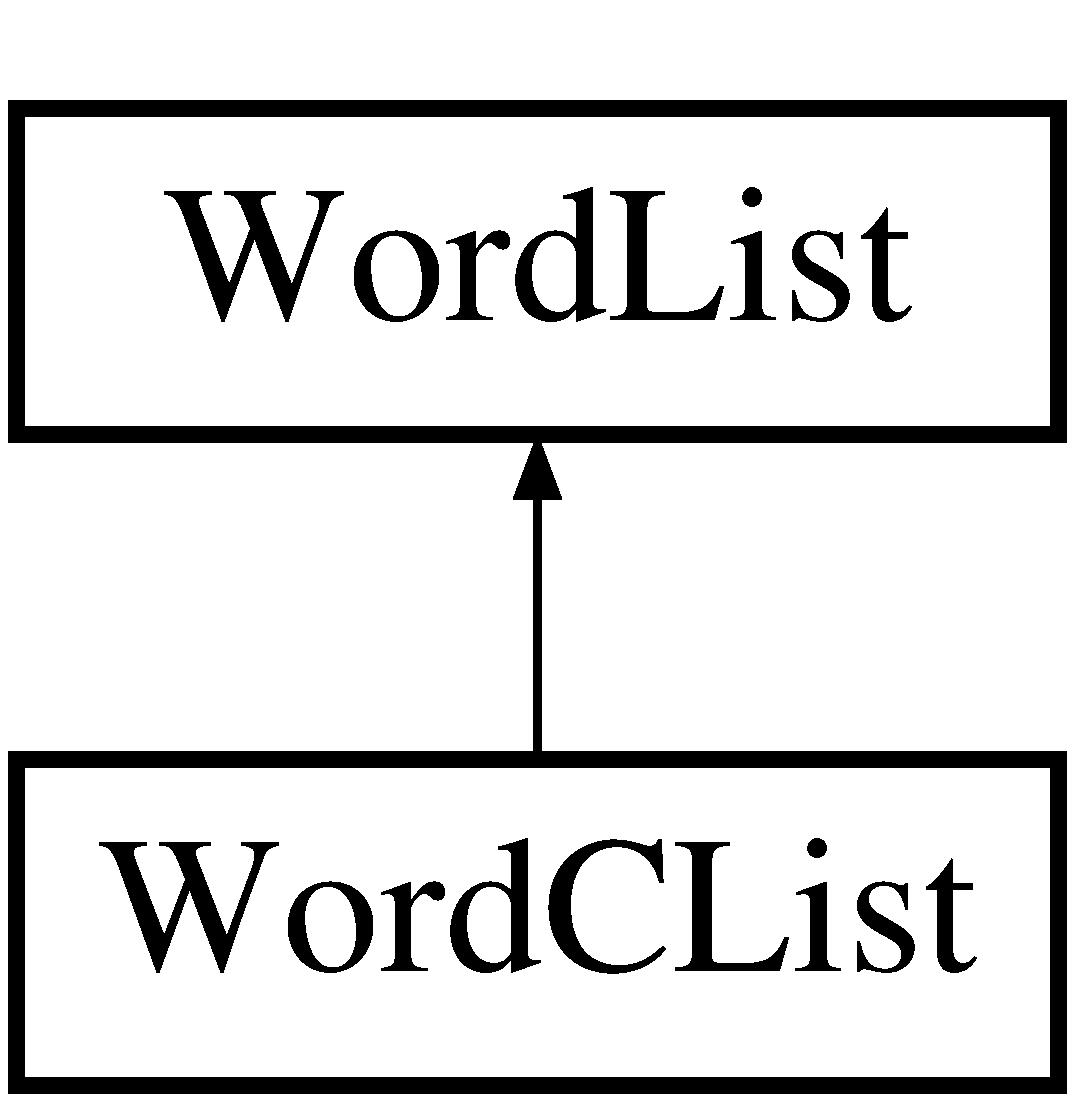
\includegraphics[height=2.000000cm]{classWordCList}
\end{center}
\end{figure}
\subsection*{Public Member Functions}
\begin{DoxyCompactItemize}
\item 
virtual void \hyperlink{classWordCList_a45ba8475164d5f5c21d9aa36183f278b}{parse\-Into\-List} (ifstream \&inf)
\begin{DoxyCompactList}\small\item\em applies polymorphism \end{DoxyCompactList}\item 
\hypertarget{classWordCList_a5aba6fc77dde7ff41f4bf4c75ba00b2c}{virtual void \hyperlink{classWordCList_a5aba6fc77dde7ff41f4bf4c75ba00b2c}{print\-Iteratively} ()}\label{classWordCList_a5aba6fc77dde7ff41f4bf4c75ba00b2c}

\begin{DoxyCompactList}\small\item\em prints the Circular Linked List using and iterator \end{DoxyCompactList}\item 
\hypertarget{classWordCList_ad4fc445b5b33b527a44e7a1245b75f8f}{virtual void \hyperlink{classWordCList_ad4fc445b5b33b527a44e7a1245b75f8f}{print\-Recursively} ()}\label{classWordCList_ad4fc445b5b33b527a44e7a1245b75f8f}

\begin{DoxyCompactList}\small\item\em prints the Circular Linked List Recursively \end{DoxyCompactList}\end{DoxyCompactItemize}


\subsection{Detailed Description}
Circular linked list subclass of \hyperlink{classWordList}{Word\-List}. 

\subsection{Member Function Documentation}
\hypertarget{classWordCList_a45ba8475164d5f5c21d9aa36183f278b}{\index{Word\-C\-List@{Word\-C\-List}!parse\-Into\-List@{parse\-Into\-List}}
\index{parse\-Into\-List@{parse\-Into\-List}!WordCList@{Word\-C\-List}}
\subsubsection[{parse\-Into\-List}]{\setlength{\rightskip}{0pt plus 5cm}void Word\-C\-List\-::parse\-Into\-List (
\begin{DoxyParamCaption}
\item[{ifstream \&}]{inf}
\end{DoxyParamCaption}
)\hspace{0.3cm}{\ttfamily [virtual]}}}\label{classWordCList_a45ba8475164d5f5c21d9aa36183f278b}


applies polymorphism 


\begin{DoxyParams}{Parameters}
{\em inf} & the file to be read from \\
\hline
\end{DoxyParams}


Implements \hyperlink{classWordList_ab91a4f01d8dac96887c7ac2c56dad2cc}{Word\-List}.



The documentation for this class was generated from the following files\-:\begin{DoxyCompactItemize}
\item 
\hyperlink{WordCList_8h}{Word\-C\-List.\-h}\item 
\hyperlink{WordCList_8cpp}{Word\-C\-List.\-cpp}\end{DoxyCompactItemize}

\hypertarget{classWordData}{\section{Word\-Data Class Reference}
\label{classWordData}\index{Word\-Data@{Word\-Data}}
}


Word Data object class containing a word and its occurence rate.  




{\ttfamily \#include $<$Word\-Data.\-h$>$}

\subsection*{Public Member Functions}
\begin{DoxyCompactItemize}
\item 
\hypertarget{classWordData_a5b4a15f68dedff06dccfa3ac69a4a144}{{\bfseries Word\-Data} (string wrd=\char`\"{}\char`\"{}, int cnt=1)}\label{classWordData_a5b4a15f68dedff06dccfa3ac69a4a144}

\item 
void \hyperlink{classWordData_ac0b321b6cc7e3d7a352e63afd6d54a36}{set\-Word} (string wrd)
\begin{DoxyCompactList}\small\item\em Sets the word. \end{DoxyCompactList}\item 
void \hyperlink{classWordData_a861d4ccae7e79af11bfb6d39ec5ee868}{set\-Count} (int cnt)
\begin{DoxyCompactList}\small\item\em Sets the occurence rate of the word. \end{DoxyCompactList}\item 
void \hyperlink{classWordData_a9e5e59a1550b3877d464ec7e1599177f}{set\-Word\-Data} (string, int)
\begin{DoxyCompactList}\small\item\em Set Whole \hyperlink{classWordData}{Word\-Data} Object. \end{DoxyCompactList}\item 
string \hyperlink{classWordData_a0002c491de4f4bd013a1b5255024a260}{get\-Word} () const 
\begin{DoxyCompactList}\small\item\em Gets the current word of the \hyperlink{classWordData}{Word\-Data} Object. \end{DoxyCompactList}\item 
int \hyperlink{classWordData_ac60a4211f9a35484ef4aaf3ddce015a0}{get\-Count} () const 
\begin{DoxyCompactList}\small\item\em Gets the occurence rate of the word. \end{DoxyCompactList}\item 
void \hyperlink{classWordData_a68428bdb3ed9b1aafa8e3aa144decec6}{inc\-Count} (int inc=1)
\begin{DoxyCompactList}\small\item\em Increment the count of the word by 1. \end{DoxyCompactList}\item 
bool \hyperlink{classWordData_a8feae3c1fd0e169b85e8a2ec613c5847}{operator$<$} (\hyperlink{classWordData}{Word\-Data})
\begin{DoxyCompactList}\small\item\em overload the $<$ operator \end{DoxyCompactList}\item 
bool \hyperlink{classWordData_a1ba05f19de8fa4a88cfad83858be4215}{operator$<$=} (\hyperlink{classWordData}{Word\-Data})
\begin{DoxyCompactList}\small\item\em overload the $<$= operator \end{DoxyCompactList}\item 
bool \hyperlink{classWordData_a6d5aed2edb9d22adac6e1b4a8c270163}{operator$>$} (\hyperlink{classWordData}{Word\-Data})
\begin{DoxyCompactList}\small\item\em overload the $>$ operator \end{DoxyCompactList}\item 
bool \hyperlink{classWordData_a6dcfbda8cee7d0c670122e565bc5d88e}{operator$>$=} (\hyperlink{classWordData}{Word\-Data})
\begin{DoxyCompactList}\small\item\em overload the $>$= operator \end{DoxyCompactList}\end{DoxyCompactItemize}


\subsection{Detailed Description}
Word Data object class containing a word and its occurence rate. 

\subsection{Member Function Documentation}
\hypertarget{classWordData_ac60a4211f9a35484ef4aaf3ddce015a0}{\index{Word\-Data@{Word\-Data}!get\-Count@{get\-Count}}
\index{get\-Count@{get\-Count}!WordData@{Word\-Data}}
\subsubsection[{get\-Count}]{\setlength{\rightskip}{0pt plus 5cm}int Word\-Data\-::get\-Count (
\begin{DoxyParamCaption}
{}
\end{DoxyParamCaption}
) const}}\label{classWordData_ac60a4211f9a35484ef4aaf3ddce015a0}


Gets the occurence rate of the word. 

\begin{DoxyReturn}{Returns}
the count 
\end{DoxyReturn}
\hypertarget{classWordData_a0002c491de4f4bd013a1b5255024a260}{\index{Word\-Data@{Word\-Data}!get\-Word@{get\-Word}}
\index{get\-Word@{get\-Word}!WordData@{Word\-Data}}
\subsubsection[{get\-Word}]{\setlength{\rightskip}{0pt plus 5cm}string Word\-Data\-::get\-Word (
\begin{DoxyParamCaption}
{}
\end{DoxyParamCaption}
) const}}\label{classWordData_a0002c491de4f4bd013a1b5255024a260}


Gets the current word of the \hyperlink{classWordData}{Word\-Data} Object. 

\begin{DoxyReturn}{Returns}
the word 
\end{DoxyReturn}
\hypertarget{classWordData_a68428bdb3ed9b1aafa8e3aa144decec6}{\index{Word\-Data@{Word\-Data}!inc\-Count@{inc\-Count}}
\index{inc\-Count@{inc\-Count}!WordData@{Word\-Data}}
\subsubsection[{inc\-Count}]{\setlength{\rightskip}{0pt plus 5cm}void Word\-Data\-::inc\-Count (
\begin{DoxyParamCaption}
\item[{int}]{inc = {\ttfamily 1}}
\end{DoxyParamCaption}
)}}\label{classWordData_a68428bdb3ed9b1aafa8e3aa144decec6}


Increment the count of the word by 1. 


\begin{DoxyParams}{Parameters}
{\em inc} & is the amount to increment by and is set to 1 \\
\hline
\end{DoxyParams}
\hypertarget{classWordData_a8feae3c1fd0e169b85e8a2ec613c5847}{\index{Word\-Data@{Word\-Data}!operator$<$@{operator$<$}}
\index{operator$<$@{operator$<$}!WordData@{Word\-Data}}
\subsubsection[{operator$<$}]{\setlength{\rightskip}{0pt plus 5cm}bool Word\-Data\-::operator$<$ (
\begin{DoxyParamCaption}
\item[{{\bf Word\-Data}}]{arg}
\end{DoxyParamCaption}
)}}\label{classWordData_a8feae3c1fd0e169b85e8a2ec613c5847}


overload the $<$ operator 


\begin{DoxyParams}{Parameters}
{\em arg} & the argument to be tested against \\
\hline
\end{DoxyParams}
\begin{DoxyReturn}{Returns}
true if $<$ arg 
\end{DoxyReturn}
\hypertarget{classWordData_a1ba05f19de8fa4a88cfad83858be4215}{\index{Word\-Data@{Word\-Data}!operator$<$=@{operator$<$=}}
\index{operator$<$=@{operator$<$=}!WordData@{Word\-Data}}
\subsubsection[{operator$<$=}]{\setlength{\rightskip}{0pt plus 5cm}bool Word\-Data\-::operator$<$= (
\begin{DoxyParamCaption}
\item[{{\bf Word\-Data}}]{arg}
\end{DoxyParamCaption}
)}}\label{classWordData_a1ba05f19de8fa4a88cfad83858be4215}


overload the $<$= operator 


\begin{DoxyParams}{Parameters}
{\em arg} & the argument to be tested against \\
\hline
\end{DoxyParams}
\begin{DoxyReturn}{Returns}
true if $<$= arg 
\end{DoxyReturn}
\hypertarget{classWordData_a6d5aed2edb9d22adac6e1b4a8c270163}{\index{Word\-Data@{Word\-Data}!operator$>$@{operator$>$}}
\index{operator$>$@{operator$>$}!WordData@{Word\-Data}}
\subsubsection[{operator$>$}]{\setlength{\rightskip}{0pt plus 5cm}bool Word\-Data\-::operator$>$ (
\begin{DoxyParamCaption}
\item[{{\bf Word\-Data}}]{arg}
\end{DoxyParamCaption}
)}}\label{classWordData_a6d5aed2edb9d22adac6e1b4a8c270163}


overload the $>$ operator 


\begin{DoxyParams}{Parameters}
{\em arg} & the argument to be tested against \\
\hline
\end{DoxyParams}
\begin{DoxyReturn}{Returns}
true if $>$ arg 
\end{DoxyReturn}
\hypertarget{classWordData_a6dcfbda8cee7d0c670122e565bc5d88e}{\index{Word\-Data@{Word\-Data}!operator$>$=@{operator$>$=}}
\index{operator$>$=@{operator$>$=}!WordData@{Word\-Data}}
\subsubsection[{operator$>$=}]{\setlength{\rightskip}{0pt plus 5cm}bool Word\-Data\-::operator$>$= (
\begin{DoxyParamCaption}
\item[{{\bf Word\-Data}}]{arg}
\end{DoxyParamCaption}
)}}\label{classWordData_a6dcfbda8cee7d0c670122e565bc5d88e}


overload the $>$= operator 


\begin{DoxyParams}{Parameters}
{\em arg} & the argument to be tested against \\
\hline
\end{DoxyParams}
\begin{DoxyReturn}{Returns}
true if $>$= arg 
\end{DoxyReturn}
\hypertarget{classWordData_a861d4ccae7e79af11bfb6d39ec5ee868}{\index{Word\-Data@{Word\-Data}!set\-Count@{set\-Count}}
\index{set\-Count@{set\-Count}!WordData@{Word\-Data}}
\subsubsection[{set\-Count}]{\setlength{\rightskip}{0pt plus 5cm}void Word\-Data\-::set\-Count (
\begin{DoxyParamCaption}
\item[{int}]{cnt}
\end{DoxyParamCaption}
)}}\label{classWordData_a861d4ccae7e79af11bfb6d39ec5ee868}


Sets the occurence rate of the word. 


\begin{DoxyParams}{Parameters}
{\em cnt} & the number of times it occurs \\
\hline
\end{DoxyParams}
\hypertarget{classWordData_ac0b321b6cc7e3d7a352e63afd6d54a36}{\index{Word\-Data@{Word\-Data}!set\-Word@{set\-Word}}
\index{set\-Word@{set\-Word}!WordData@{Word\-Data}}
\subsubsection[{set\-Word}]{\setlength{\rightskip}{0pt plus 5cm}void Word\-Data\-::set\-Word (
\begin{DoxyParamCaption}
\item[{string}]{wrd}
\end{DoxyParamCaption}
)}}\label{classWordData_ac0b321b6cc7e3d7a352e63afd6d54a36}


Sets the word. 


\begin{DoxyParams}{Parameters}
{\em wrd} & the word to be set \\
\hline
\end{DoxyParams}
\hypertarget{classWordData_a9e5e59a1550b3877d464ec7e1599177f}{\index{Word\-Data@{Word\-Data}!set\-Word\-Data@{set\-Word\-Data}}
\index{set\-Word\-Data@{set\-Word\-Data}!WordData@{Word\-Data}}
\subsubsection[{set\-Word\-Data}]{\setlength{\rightskip}{0pt plus 5cm}void Word\-Data\-::set\-Word\-Data (
\begin{DoxyParamCaption}
\item[{string}]{wrd, }
\item[{int}]{cnt}
\end{DoxyParamCaption}
)}}\label{classWordData_a9e5e59a1550b3877d464ec7e1599177f}


Set Whole \hyperlink{classWordData}{Word\-Data} Object. 


\begin{DoxyParams}{Parameters}
{\em wrd} & the word to be set \\
\hline
{\em cnt} & the number of times it occurs \\
\hline
\end{DoxyParams}


The documentation for this class was generated from the following files\-:\begin{DoxyCompactItemize}
\item 
\hyperlink{WordData_8h}{Word\-Data.\-h}\item 
\hyperlink{WordData_8cpp}{Word\-Data.\-cpp}\end{DoxyCompactItemize}

\hypertarget{classWordDataList}{\section{Word\-Data\-List Class Reference}
\label{classWordDataList}\index{Word\-Data\-List@{Word\-Data\-List}}
}
Inheritance diagram for Word\-Data\-List\-:\begin{figure}[H]
\begin{center}
\leavevmode
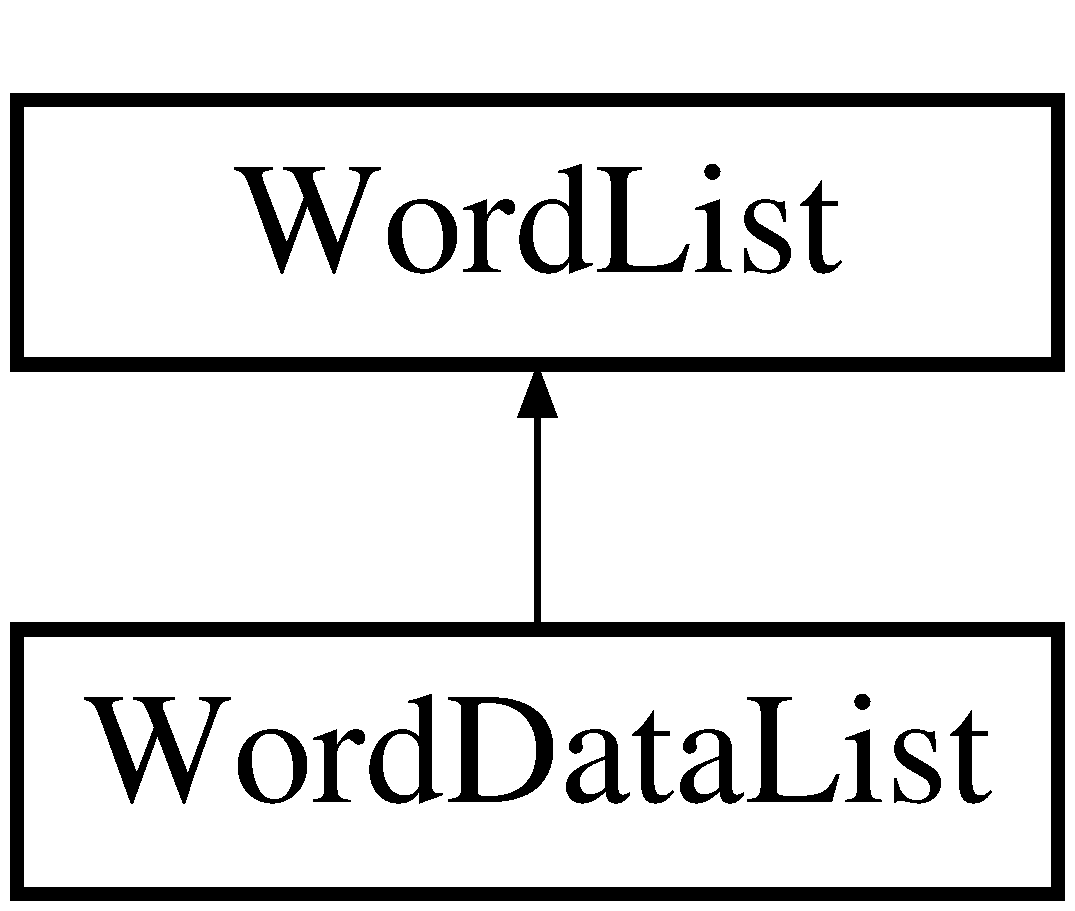
\includegraphics[height=2.000000cm]{classWordDataList}
\end{center}
\end{figure}
\subsection*{Public Member Functions}
\begin{DoxyCompactItemize}
\item 
virtual void \hyperlink{classWordDataList_a5408e39b6c4c58e0d21463560ee60cd0}{parse\-Into\-List} (ifstream \&inf)
\begin{DoxyCompactList}\small\item\em applies polymorphism \end{DoxyCompactList}\item 
\hypertarget{classWordDataList_aec2c3363ab94af00c6bce272c04358d2}{virtual void \hyperlink{classWordDataList_aec2c3363ab94af00c6bce272c04358d2}{print\-Iteratively} ()}\label{classWordDataList_aec2c3363ab94af00c6bce272c04358d2}

\begin{DoxyCompactList}\small\item\em Print the data iteratively. \end{DoxyCompactList}\item 
\hypertarget{classWordDataList_a40afa65c3afcd1f96e887de858914b83}{virtual void \hyperlink{classWordDataList_a40afa65c3afcd1f96e887de858914b83}{print\-Recursively} ()}\label{classWordDataList_a40afa65c3afcd1f96e887de858914b83}

\begin{DoxyCompactList}\small\item\em Call worker function to print the data recursively. \end{DoxyCompactList}\item 
\hypertarget{classWordDataList_a9406a5f004ebe03d09851fbe8b2b827d}{virtual void \hyperlink{classWordDataList_a9406a5f004ebe03d09851fbe8b2b827d}{print\-Ptr\-Recursively} ()}\label{classWordDataList_a9406a5f004ebe03d09851fbe8b2b827d}

\begin{DoxyCompactList}\small\item\em Call worker function to print the data recursively. \end{DoxyCompactList}\end{DoxyCompactItemize}


\subsection{Member Function Documentation}
\hypertarget{classWordDataList_a5408e39b6c4c58e0d21463560ee60cd0}{\index{Word\-Data\-List@{Word\-Data\-List}!parse\-Into\-List@{parse\-Into\-List}}
\index{parse\-Into\-List@{parse\-Into\-List}!WordDataList@{Word\-Data\-List}}
\subsubsection[{parse\-Into\-List}]{\setlength{\rightskip}{0pt plus 5cm}void Word\-Data\-List\-::parse\-Into\-List (
\begin{DoxyParamCaption}
\item[{ifstream \&}]{inf}
\end{DoxyParamCaption}
)\hspace{0.3cm}{\ttfamily [virtual]}}}\label{classWordDataList_a5408e39b6c4c58e0d21463560ee60cd0}


applies polymorphism 


\begin{DoxyParams}{Parameters}
{\em inf} & the file to be read from \\
\hline
\end{DoxyParams}


Implements \hyperlink{classWordList_ab91a4f01d8dac96887c7ac2c56dad2cc}{Word\-List}.



The documentation for this class was generated from the following files\-:\begin{DoxyCompactItemize}
\item 
\hyperlink{WordDataList_8h}{Word\-Data\-List.\-h}\item 
\hyperlink{WordDataList_8cpp}{Word\-Data\-List.\-cpp}\end{DoxyCompactItemize}

\hypertarget{classWordList}{\section{Word\-List Class Reference}
\label{classWordList}\index{Word\-List@{Word\-List}}
}


base class for containers of word data  




{\ttfamily \#include $<$Word\-List.\-h$>$}

Inheritance diagram for Word\-List\-:\begin{figure}[H]
\begin{center}
\leavevmode
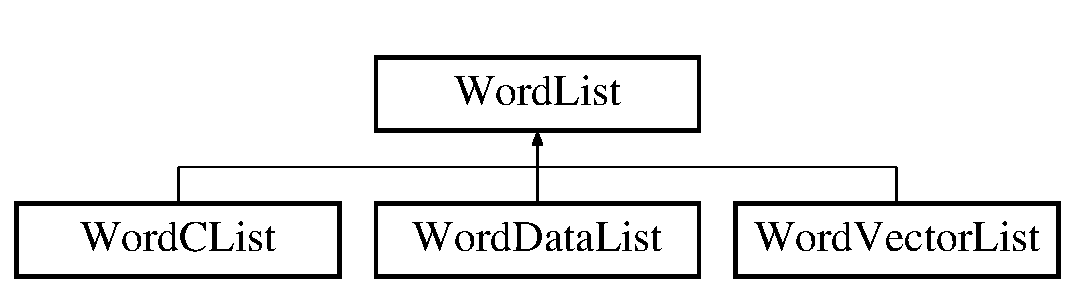
\includegraphics[height=2.000000cm]{classWordList}
\end{center}
\end{figure}
\subsection*{Public Member Functions}
\begin{DoxyCompactItemize}
\item 
virtual void \hyperlink{classWordList_ab91a4f01d8dac96887c7ac2c56dad2cc}{parse\-Into\-List} (ifstream \&inf)=0
\begin{DoxyCompactList}\small\item\em applies polymorphism \end{DoxyCompactList}\item 
\hypertarget{classWordList_a26badccde80f7083b20b3ff66879277a}{virtual void \hyperlink{classWordList_a26badccde80f7083b20b3ff66879277a}{print\-Iteratively} ()=0}\label{classWordList_a26badccde80f7083b20b3ff66879277a}

\begin{DoxyCompactList}\small\item\em prints the Circular Linked List using and iterator \end{DoxyCompactList}\item 
\hypertarget{classWordList_af016ca3e7c27bf683df412ff54557ac3}{virtual void \hyperlink{classWordList_af016ca3e7c27bf683df412ff54557ac3}{print\-Recursively} ()=0}\label{classWordList_af016ca3e7c27bf683df412ff54557ac3}

\begin{DoxyCompactList}\small\item\em prints the Circular Linked List Recursively \end{DoxyCompactList}\item 
\hypertarget{classWordList_a4f1eaa87c656cce3a2a98c5a7285da98}{virtual void \hyperlink{classWordList_a4f1eaa87c656cce3a2a98c5a7285da98}{print\-Ptr\-Recursively} ()}\label{classWordList_a4f1eaa87c656cce3a2a98c5a7285da98}

\begin{DoxyCompactList}\small\item\em Call worker function to print the data recursively. \end{DoxyCompactList}\end{DoxyCompactItemize}


\subsection{Detailed Description}
base class for containers of word data 

\subsection{Member Function Documentation}
\hypertarget{classWordList_ab91a4f01d8dac96887c7ac2c56dad2cc}{\index{Word\-List@{Word\-List}!parse\-Into\-List@{parse\-Into\-List}}
\index{parse\-Into\-List@{parse\-Into\-List}!WordList@{Word\-List}}
\subsubsection[{parse\-Into\-List}]{\setlength{\rightskip}{0pt plus 5cm}virtual void Word\-List\-::parse\-Into\-List (
\begin{DoxyParamCaption}
\item[{ifstream \&}]{inf}
\end{DoxyParamCaption}
)\hspace{0.3cm}{\ttfamily [pure virtual]}}}\label{classWordList_ab91a4f01d8dac96887c7ac2c56dad2cc}


applies polymorphism 


\begin{DoxyParams}{Parameters}
{\em inf} & the file to be read from \\
\hline
\end{DoxyParams}


Implemented in \hyperlink{classWordCList_a45ba8475164d5f5c21d9aa36183f278b}{Word\-C\-List}, \hyperlink{classWordDataList_a5408e39b6c4c58e0d21463560ee60cd0}{Word\-Data\-List}, and \hyperlink{classWordVectorList_a5c34565d237b25447223ba857ee6d181}{Word\-Vector\-List}.



The documentation for this class was generated from the following file\-:\begin{DoxyCompactItemize}
\item 
\hyperlink{WordList_8h}{Word\-List.\-h}\end{DoxyCompactItemize}

\hypertarget{classWordVectorList}{\section{Word\-Vector\-List Class Reference}
\label{classWordVectorList}\index{Word\-Vector\-List@{Word\-Vector\-List}}
}


vector list subclass of \hyperlink{classWordList}{Word\-List}  




{\ttfamily \#include $<$Word\-Vector\-List.\-h$>$}

Inheritance diagram for Word\-Vector\-List\-:\begin{figure}[H]
\begin{center}
\leavevmode
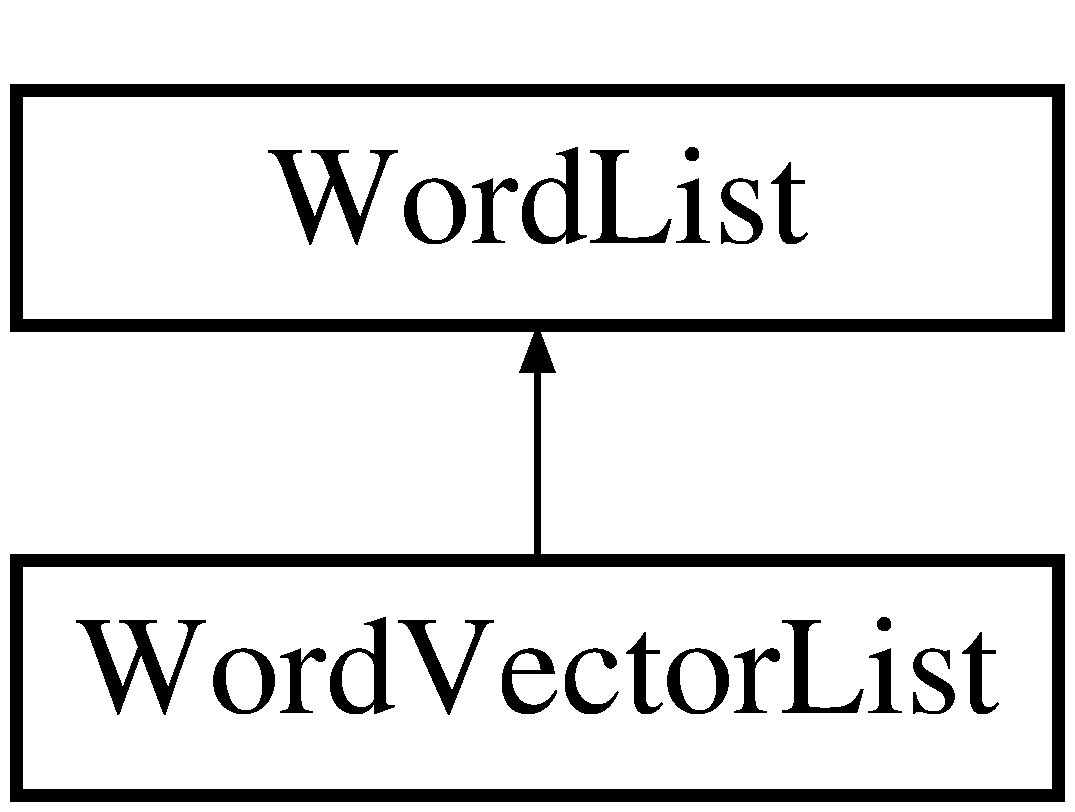
\includegraphics[height=2.000000cm]{classWordVectorList}
\end{center}
\end{figure}
\subsection*{Public Member Functions}
\begin{DoxyCompactItemize}
\item 
virtual void \hyperlink{classWordVectorList_a5c34565d237b25447223ba857ee6d181}{parse\-Into\-List} (ifstream \&inf)
\begin{DoxyCompactList}\small\item\em applies polymorphism \end{DoxyCompactList}\item 
\hypertarget{classWordVectorList_aaca0c4541139739a209901d234e2af11}{virtual void \hyperlink{classWordVectorList_aaca0c4541139739a209901d234e2af11}{print\-Iteratively} ()}\label{classWordVectorList_aaca0c4541139739a209901d234e2af11}

\begin{DoxyCompactList}\small\item\em prints the vector List using and iterator \end{DoxyCompactList}\item 
\hypertarget{classWordVectorList_ae76eba4758b69d9c7efb433555971f2f}{virtual void \hyperlink{classWordVectorList_ae76eba4758b69d9c7efb433555971f2f}{print\-Recursively} ()}\label{classWordVectorList_ae76eba4758b69d9c7efb433555971f2f}

\begin{DoxyCompactList}\small\item\em prints the vector List Recursively \end{DoxyCompactList}\end{DoxyCompactItemize}


\subsection{Detailed Description}
vector list subclass of \hyperlink{classWordList}{Word\-List} 

\subsection{Member Function Documentation}
\hypertarget{classWordVectorList_a5c34565d237b25447223ba857ee6d181}{\index{Word\-Vector\-List@{Word\-Vector\-List}!parse\-Into\-List@{parse\-Into\-List}}
\index{parse\-Into\-List@{parse\-Into\-List}!WordVectorList@{Word\-Vector\-List}}
\subsubsection[{parse\-Into\-List}]{\setlength{\rightskip}{0pt plus 5cm}void Word\-Vector\-List\-::parse\-Into\-List (
\begin{DoxyParamCaption}
\item[{ifstream \&}]{inf}
\end{DoxyParamCaption}
)\hspace{0.3cm}{\ttfamily [virtual]}}}\label{classWordVectorList_a5c34565d237b25447223ba857ee6d181}


applies polymorphism 


\begin{DoxyParams}{Parameters}
{\em inf} & the file to be read from \\
\hline
\end{DoxyParams}


Implements \hyperlink{classWordList_ab91a4f01d8dac96887c7ac2c56dad2cc}{Word\-List}.



The documentation for this class was generated from the following files\-:\begin{DoxyCompactItemize}
\item 
\hyperlink{WordVectorList_8h}{Word\-Vector\-List.\-h}\item 
\hyperlink{WordVectorList_8cpp}{Word\-Vector\-List.\-cpp}\end{DoxyCompactItemize}

\chapter{File Documentation}
\hypertarget{app_8cpp}{\section{app.\-cpp File Reference}
\label{app_8cpp}\index{app.\-cpp@{app.\-cpp}}
}


test driver for Project3  


{\ttfamily \#include $<$iostream$>$}\\*
{\ttfamily \#include $<$sstream$>$}\\*
{\ttfamily \#include $<$vector$>$}\\*
{\ttfamily \#include $<$fstream$>$}\\*
{\ttfamily \#include \char`\"{}Word\-List.\-h\char`\"{}}\\*
{\ttfamily \#include \char`\"{}Word\-Data\-List.\-h\char`\"{}}\\*
{\ttfamily \#include \char`\"{}Word\-Vector\-List.\-h\char`\"{}}\\*
{\ttfamily \#include \char`\"{}Word\-C\-List.\-h\char`\"{}}\\*
{\ttfamily \#include $<$chrono$>$}\\*
\subsection*{Functions}
\begin{DoxyCompactItemize}
\item 
\hypertarget{app_8cpp_a59c2926dd9b0968badf463aaf4f91422}{void \hyperlink{app_8cpp_a59c2926dd9b0968badf463aaf4f91422}{display\-Menu} ()}\label{app_8cpp_a59c2926dd9b0968badf463aaf4f91422}

\begin{DoxyCompactList}\small\item\em prints out the menu \end{DoxyCompactList}\item 
void \hyperlink{app_8cpp_a3b1e899508b02472932875555e64cd16}{print\-Everything} (ifstream \&inf, \hyperlink{classWordList}{Word\-List} $\ast$The\-List)
\begin{DoxyCompactList}\small\item\em Prints out all options. \end{DoxyCompactList}\item 
\hypertarget{app_8cpp_a0ddf1224851353fc92bfbff6f499fa97}{int {\bfseries main} (int argc, char $\ast$argv\mbox{[}$\,$\mbox{]})}\label{app_8cpp_a0ddf1224851353fc92bfbff6f499fa97}

\end{DoxyCompactItemize}


\subsection{Detailed Description}
test driver for Project3 

\subsection{Function Documentation}
\hypertarget{app_8cpp_a3b1e899508b02472932875555e64cd16}{\index{app.\-cpp@{app.\-cpp}!print\-Everything@{print\-Everything}}
\index{print\-Everything@{print\-Everything}!app.cpp@{app.\-cpp}}
\subsubsection[{print\-Everything}]{\setlength{\rightskip}{0pt plus 5cm}void print\-Everything (
\begin{DoxyParamCaption}
\item[{ifstream \&}]{inf, }
\item[{{\bf Word\-List} $\ast$}]{The\-List}
\end{DoxyParamCaption}
)}}\label{app_8cpp_a3b1e899508b02472932875555e64cd16}


Prints out all options. 


\begin{DoxyParams}{Parameters}
{\em inf} & the file to be read from \\
\hline
{\em The\-List} & a pointer to a \hyperlink{classWordList}{Word\-List} that is pointed at a \hyperlink{classWordList}{Word\-List} subclass \\
\hline
\end{DoxyParams}

\hypertarget{WordCList_8cpp}{\section{Word\-C\-List.\-cpp File Reference}
\label{WordCList_8cpp}\index{Word\-C\-List.\-cpp@{Word\-C\-List.\-cpp}}
}


file for the \hyperlink{classWordCList}{Word\-C\-List} subclass implemenation  


{\ttfamily \#include $<$sstream$>$}\\*
{\ttfamily \#include $<$iostream$>$}\\*
{\ttfamily \#include \char`\"{}Word\-C\-List.\-h\char`\"{}}\\*
{\ttfamily \#include \char`\"{}Linked\-List.\-h\char`\"{}}\\*


\subsection{Detailed Description}
file for the \hyperlink{classWordCList}{Word\-C\-List} subclass implemenation 
\hypertarget{WordCList_8h}{\section{Word\-C\-List.\-h File Reference}
\label{WordCList_8h}\index{Word\-C\-List.\-h@{Word\-C\-List.\-h}}
}


header file for the \hyperlink{classWordCList}{Word\-C\-List} subclass  


{\ttfamily \#include $<$assert.\-h$>$}\\*
{\ttfamily \#include $<$iostream$>$}\\*
{\ttfamily \#include \char`\"{}Word\-List.\-h\char`\"{}}\\*
{\ttfamily \#include \char`\"{}Word\-Data.\-h\char`\"{}}\\*
{\ttfamily \#include \char`\"{}Linked\-List.\-h\char`\"{}}\\*
\subsection*{Classes}
\begin{DoxyCompactItemize}
\item 
class \hyperlink{classWordCList}{Word\-C\-List}
\begin{DoxyCompactList}\small\item\em Circular linked list subclass of \hyperlink{classWordList}{Word\-List}. \end{DoxyCompactList}\end{DoxyCompactItemize}


\subsection{Detailed Description}
header file for the \hyperlink{classWordCList}{Word\-C\-List} subclass 
\hypertarget{WordData_8cpp}{\section{Word\-Data.\-cpp File Reference}
\label{WordData_8cpp}\index{Word\-Data.\-cpp@{Word\-Data.\-cpp}}
}


file for the \hyperlink{classWordData}{Word\-Data} Class object implementation  


{\ttfamily \#include $<$iostream$>$}\\*
{\ttfamily \#include $<$iomanip$>$}\\*
{\ttfamily \#include $<$sstream$>$}\\*
{\ttfamily \#include $<$string$>$}\\*
{\ttfamily \#include \char`\"{}Word\-Data.\-h\char`\"{}}\\*
\subsection*{Functions}
\begin{DoxyCompactItemize}
\item 
ostream \& \hyperlink{WordData_8cpp_a5cc8d7bcdce0d214770dabd858b0bd82}{operator$<$$<$} (ostream \&output, const \hyperlink{classWordData}{Word\-Data} \&words)
\begin{DoxyCompactList}\small\item\em overload operator for output \end{DoxyCompactList}\end{DoxyCompactItemize}


\subsection{Detailed Description}
file for the \hyperlink{classWordData}{Word\-Data} Class object implementation 

\subsection{Function Documentation}
\hypertarget{WordData_8cpp_a5cc8d7bcdce0d214770dabd858b0bd82}{\index{Word\-Data.\-cpp@{Word\-Data.\-cpp}!operator$<$$<$@{operator$<$$<$}}
\index{operator$<$$<$@{operator$<$$<$}!WordData.cpp@{Word\-Data.\-cpp}}
\subsubsection[{operator$<$$<$}]{\setlength{\rightskip}{0pt plus 5cm}ostream\& operator$<$$<$ (
\begin{DoxyParamCaption}
\item[{ostream \&}]{output, }
\item[{const {\bf Word\-Data} \&}]{words}
\end{DoxyParamCaption}
)}}\label{WordData_8cpp_a5cc8d7bcdce0d214770dabd858b0bd82}


overload operator for output 


\begin{DoxyParams}{Parameters}
{\em output} & is the output stream \\
\hline
{\em words} & is the \hyperlink{classWordData}{Word\-Data} \\
\hline
\end{DoxyParams}
\begin{DoxyReturn}{Returns}
the output stream 
\end{DoxyReturn}

\hypertarget{WordData_8h}{\section{Word\-Data.\-h File Reference}
\label{WordData_8h}\index{Word\-Data.\-h@{Word\-Data.\-h}}
}


header file for the \hyperlink{classWordData}{Word\-Data} Class  


{\ttfamily \#include $<$iostream$>$}\\*
{\ttfamily \#include $<$string$>$}\\*
\subsection*{Classes}
\begin{DoxyCompactItemize}
\item 
class \hyperlink{classWordData}{Word\-Data}
\begin{DoxyCompactList}\small\item\em Word Data object class containing a word and its occurence rate. \end{DoxyCompactList}\end{DoxyCompactItemize}
\subsection*{Functions}
\begin{DoxyCompactItemize}
\item 
ostream \& \hyperlink{WordData_8h_a5cc8d7bcdce0d214770dabd858b0bd82}{operator$<$$<$} (ostream \&output, const \hyperlink{classWordData}{Word\-Data} \&words)
\begin{DoxyCompactList}\small\item\em overload operator for output \end{DoxyCompactList}\end{DoxyCompactItemize}


\subsection{Detailed Description}
header file for the \hyperlink{classWordData}{Word\-Data} Class 

\subsection{Function Documentation}
\hypertarget{WordData_8h_a5cc8d7bcdce0d214770dabd858b0bd82}{\index{Word\-Data.\-h@{Word\-Data.\-h}!operator$<$$<$@{operator$<$$<$}}
\index{operator$<$$<$@{operator$<$$<$}!WordData.h@{Word\-Data.\-h}}
\subsubsection[{operator$<$$<$}]{\setlength{\rightskip}{0pt plus 5cm}ostream\& operator$<$$<$ (
\begin{DoxyParamCaption}
\item[{ostream \&}]{output, }
\item[{const {\bf Word\-Data} \&}]{words}
\end{DoxyParamCaption}
)}}\label{WordData_8h_a5cc8d7bcdce0d214770dabd858b0bd82}


overload operator for output 


\begin{DoxyParams}{Parameters}
{\em output} & is the output stream \\
\hline
{\em words} & is the \hyperlink{classWordData}{Word\-Data} \\
\hline
\end{DoxyParams}
\begin{DoxyReturn}{Returns}
the output stream 
\end{DoxyReturn}

\hypertarget{WordDataList_8cpp}{\section{Word\-Data\-List.\-cpp File Reference}
\label{WordDataList_8cpp}\index{Word\-Data\-List.\-cpp@{Word\-Data\-List.\-cpp}}
}


Container of \hyperlink{classWordData}{Word\-Data} objects.  


{\ttfamily \#include $<$sstream$>$}\\*
{\ttfamily \#include $<$iostream$>$}\\*
{\ttfamily \#include \char`\"{}Word\-Data\-List.\-h\char`\"{}}\\*


\subsection{Detailed Description}
Container of \hyperlink{classWordData}{Word\-Data} objects. 
\hypertarget{WordDataList_8h}{\section{Word\-Data\-List.\-h File Reference}
\label{WordDataList_8h}\index{Word\-Data\-List.\-h@{Word\-Data\-List.\-h}}
}


Container of \hyperlink{classWordData}{Word\-Data} objects.  


{\ttfamily \#include $<$string$>$}\\*
{\ttfamily \#include \char`\"{}Word\-List.\-h\char`\"{}}\\*
{\ttfamily \#include \char`\"{}Word\-Data.\-h\char`\"{}}\\*
\subsection*{Classes}
\begin{DoxyCompactItemize}
\item 
class \hyperlink{classWordDataList}{Word\-Data\-List}
\end{DoxyCompactItemize}


\subsection{Detailed Description}
Container of \hyperlink{classWordData}{Word\-Data} objects. 
\hypertarget{WordList_8h}{\section{Word\-List.\-h File Reference}
\label{WordList_8h}\index{Word\-List.\-h@{Word\-List.\-h}}
}


Abstract base class for containers of word data.  


{\ttfamily \#include $<$fstream$>$}\\*
{\ttfamily \#include $<$string$>$}\\*
\subsection*{Classes}
\begin{DoxyCompactItemize}
\item 
class \hyperlink{classWordList}{Word\-List}
\begin{DoxyCompactList}\small\item\em base class for containers of word data \end{DoxyCompactList}\end{DoxyCompactItemize}


\subsection{Detailed Description}
Abstract base class for containers of word data. 
\hypertarget{WordVectorList_8cpp}{\section{Word\-Vector\-List.\-cpp File Reference}
\label{WordVectorList_8cpp}\index{Word\-Vector\-List.\-cpp@{Word\-Vector\-List.\-cpp}}
}


file for the \hyperlink{classWordVectorList}{Word\-Vector\-List} subclass implemenation  


{\ttfamily \#include $<$sstream$>$}\\*
{\ttfamily \#include $<$iostream$>$}\\*
{\ttfamily \#include $<$algorithm$>$}\\*
{\ttfamily \#include \char`\"{}Word\-Vector\-List.\-h\char`\"{}}\\*


\subsection{Detailed Description}
file for the \hyperlink{classWordVectorList}{Word\-Vector\-List} subclass implemenation 
\hypertarget{WordVectorList_8h}{\section{Word\-Vector\-List.\-h File Reference}
\label{WordVectorList_8h}\index{Word\-Vector\-List.\-h@{Word\-Vector\-List.\-h}}
}


header file for the \hyperlink{classWordVectorList}{Word\-Vector\-List} subclass  


{\ttfamily \#include $<$vector$>$}\\*
{\ttfamily \#include \char`\"{}Word\-List.\-h\char`\"{}}\\*
{\ttfamily \#include \char`\"{}Word\-Data.\-h\char`\"{}}\\*
\subsection*{Classes}
\begin{DoxyCompactItemize}
\item 
class \hyperlink{classWordVectorList}{Word\-Vector\-List}
\begin{DoxyCompactList}\small\item\em vector list subclass of \hyperlink{classWordList}{Word\-List} \end{DoxyCompactList}\end{DoxyCompactItemize}


\subsection{Detailed Description}
header file for the \hyperlink{classWordVectorList}{Word\-Vector\-List} subclass 
%--- End generated contents ---

% Index
\newpage
\phantomsection
\addcontentsline{toc}{part}{Index}
\printindex

\end{document}
